\renewcommand{\FileName}{mreg}
% slide template
\begin{frame}
  \frametitle{HE plots for Multivariate Multiple Regression}
  \begin{itemize}
  	\item<1->{\large\bfseries Model}: $\mat{Y} = \mat{X} \mat{B} + \mat{U}$, where cols of $\mat{X}$ are
	quantitative.
	\item<1->{\large\bfseries Overall test}: $H_0: \mat{B} = \mat{0}$ (all coefficients
for all responses are zero)
      \begin{itemize*}
	  \item $\rightarrow \mat{C} = \mat{I}$ in GLT $\rightarrow
\mat{H}  =
 \widehat{\mat{B}}\trans \,
 (\mat{X}\trans \mat{X} )^{-1} \,
 \widehat{\mat{B}}
 =  \widehat{\mat{Y}}\trans \, \widehat{\mat{Y}}$
	  \end{itemize*}
	\item<1->{\large\bfseries Individual predictors}: $H_0 : \vec{\beta}_i = \vec{0}$
      \begin{itemize*}
	  \item $\rightarrow \mat{C} = (0, 0, \dots, 1 , 0, \dots, 0)\rightarrow
	  	\mat{H}_i = \hat{\vec{\beta}}_i \trans (\mat{X}\trans \mat{X} )^{-1}
\hat{\vec{\beta}}_i $
      \end{itemize*}
	\item<2->{\large\bfseries HE plot}
      \begin{itemize*}
	    \item Overall \H ellipse: how predictors relate collectively to responses
		\item Individual \H ellipses (rank(\H)=1 $\rightarrow$ vectors):
		\begin{itemize*}
		  \item orientation $\rightarrow$ relation of $\vec{x}_i$ to $\vec{y}_1, \vec{y}_2$
%		  \item angles $\rightarrow$ relation of $\vec{x}_i$ to $\vec{y}_1, \vec{y}_2$
		  \item length $\rightarrow$ strength of relation
		  \item collection of individual \H vectors $\rightarrow$ how predictors contribute to
		  overall test.
		\end{itemize*}
      \end{itemize*}
  \end{itemize}

\end{frame}

\begin{frame}[plain]
  \frametitle{HE plots for MMRA: Example}
  \begin{itemize*}
	\item Rohwer data on $n=37$ low SES children, for 5 PA tasks (N, S, NS, NA, SS) predicting
	intelligence/achievement (PPVT, SAT, Raven)
  \end{itemize*}
  \begin{columns}
    \begin{column}[T]{.4\textwidth}
	  \begin{itemize}
	    \item<1-> Only NA is individually significant (in this view)
		\item<1-> $\dots$ but overall test highly significant
		\item<2-> NA \& S contribute to predicting PPVT
		\item<2-> NS \& SS contribute to predicting SAT
	  \end{itemize}
    \end{column}
    \begin{column}[T]{.6\textwidth}
	  \includegraphics[width=.85\textwidth,clip]{fig/mreg6}
    \end{column}
  \end{columns}
\end{frame}

\mode<\inlong>{
\begin{frame}[plain]
  \frametitle{HE plots for MMRA: Example}
  For any model term:
  \begin{itemize*}
  	\item<1->\H ellipse: covariation of fitted values
  	\item<2->\red{\E ellipse: covariation of residuals}
	\item<3>shift, scale, overlay
  \end{itemize*}
  \begin{columns}
  	\begin{column}[t]{.5\textwidth}
	  \includegraphics<1-2>[width=\textwidth,clip]{fig/mreg3a1}
	\end{column}
  	\begin{column}[t]{.5\textwidth}
	  \includegraphics<2>[width=\textwidth,clip]{fig/mreg3a2}
	\end{column}
  \end{columns}
  \begin{center}
	  \includegraphics<3>[width=.5\textwidth,clip]{fig/mreg3a4}
  \end{center}
\end{frame}
}

%\begin{frame}
%  \frametitle{HE plots for MMRA: MANCOVA}
%  \begin{itemize*}
%	\item Rohwer data on $n_1=37$ low SES, and $n_2=32$ high SES children
%	\begin{itemize*}
%%	  \item Are regressions parallel?  Are they coincident?
%	  \item Fit separate regressions for each group
%	\end{itemize*}
%  \end{itemize*}
%\begin{center}
%  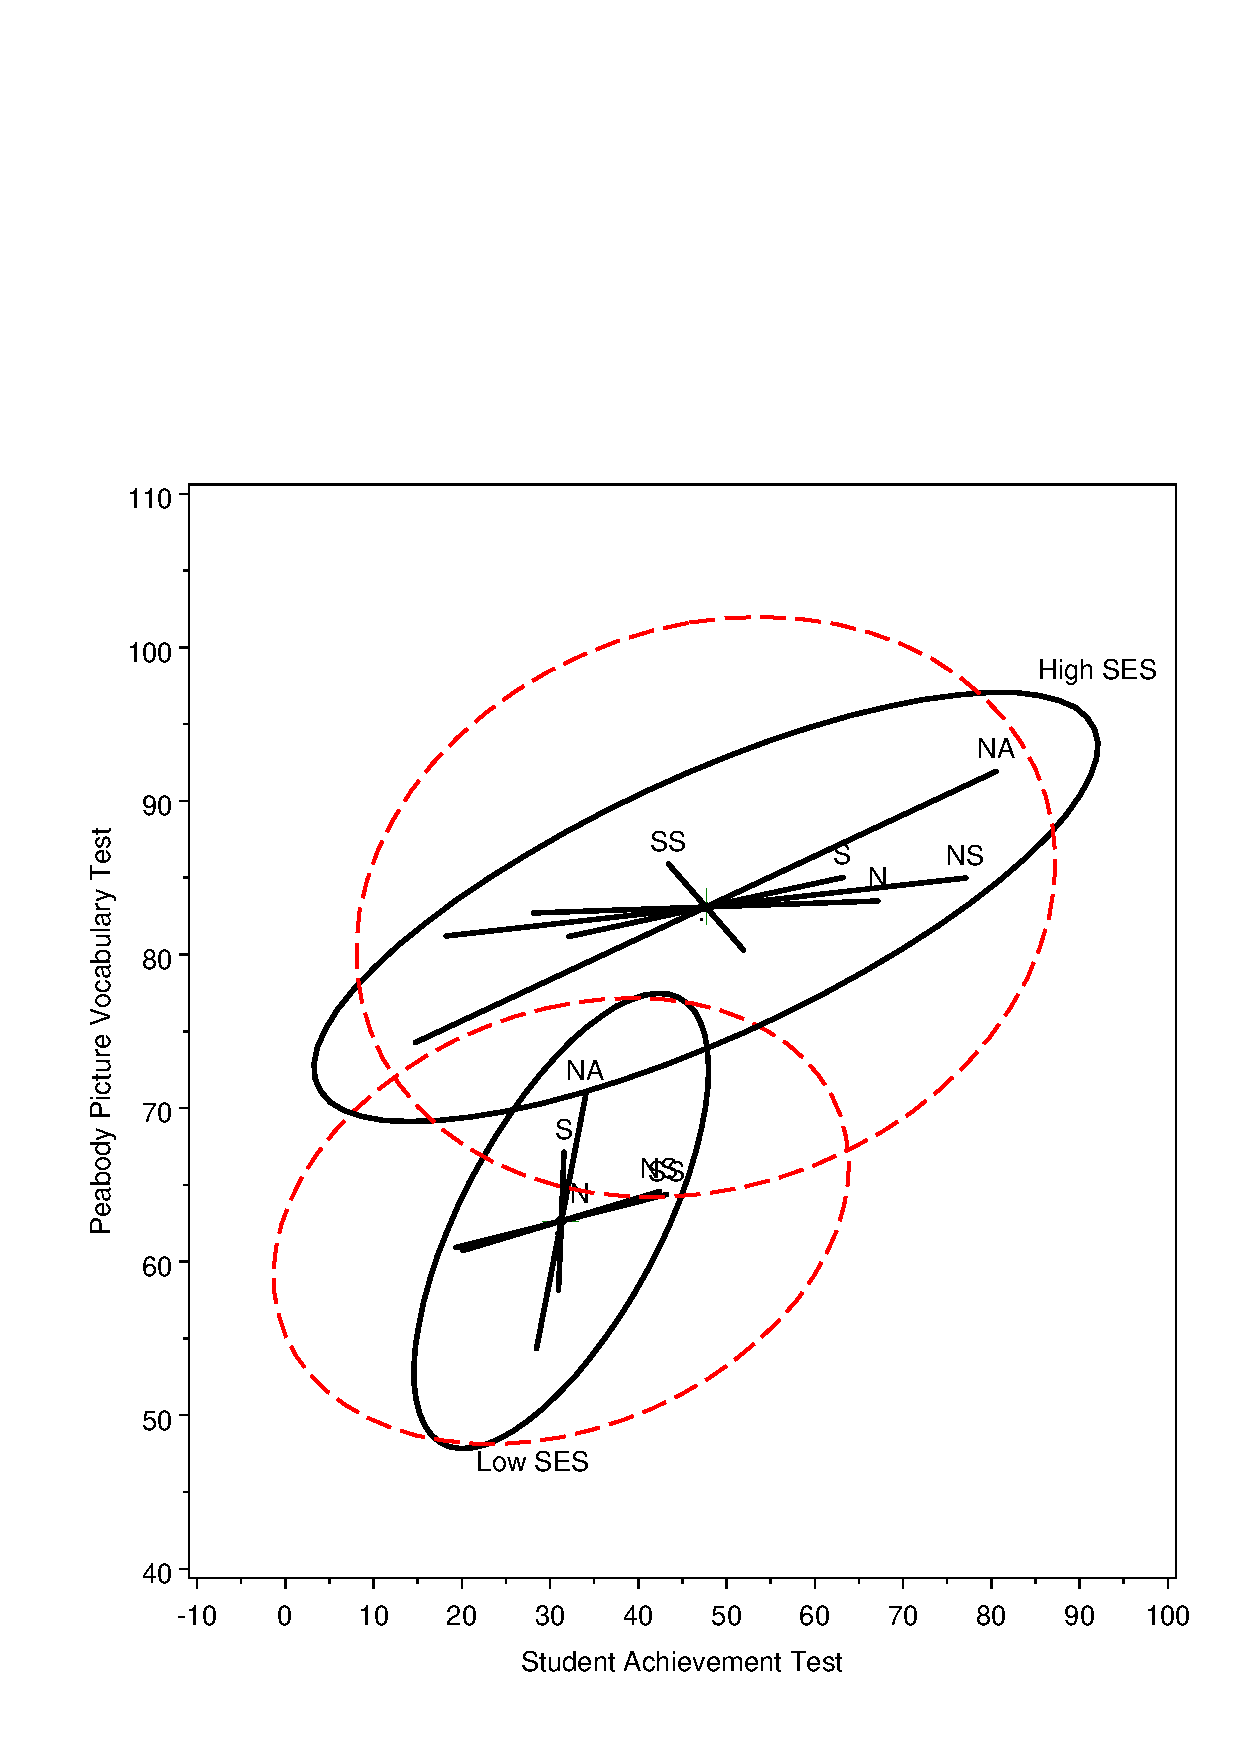
\includegraphics[height=.75\textheight,clip]{fig/mreg5}
%\end{center}
%\end{frame}

\begin{frame}
  \frametitle{HE plots for MMRA: MANCOVA}
  \begin{itemize*}
	\item Rohwer data on $n_1=37$ low SES, and $n_2=32$ high SES children
  \end{itemize*}
  \begin{columns}
  	\begin{column}[T]{.4\textwidth}
	\begin{itemize*}
	  \item Are regressions parallel?  
	  \item Are they coincident?
	  \item Fit separate regressions for each group
	\end{itemize*}
	\end{column}
  	\begin{column}[T]{.6\textwidth}
%	  \includegraphics<2->[width=\textwidth,clip]{fig/mreg3a2}
	  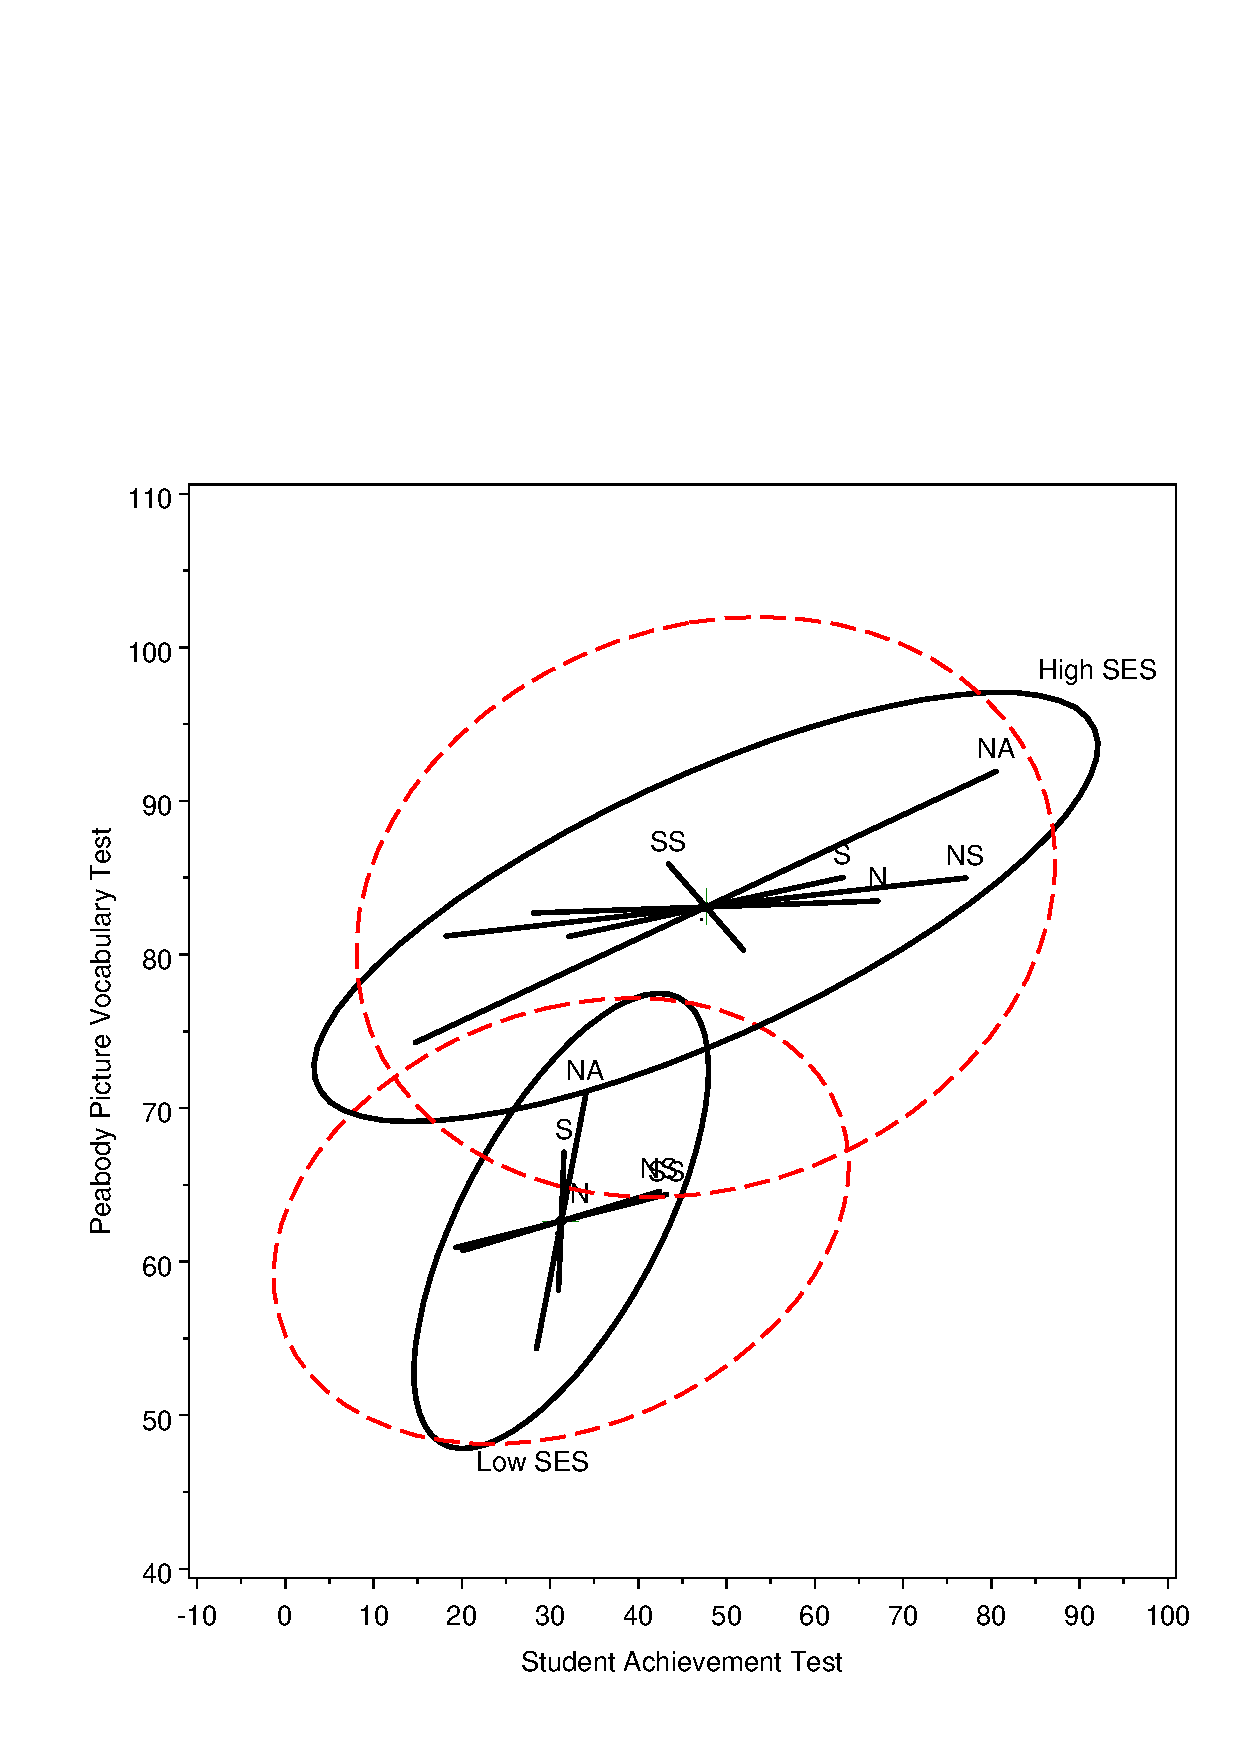
\includegraphics[width=.95\textwidth,clip]{fig/mreg5}
	\end{column}
  \end{columns}
\end{frame}

\begin{frame}
  \frametitle{HE plots for MMRA: MANCOVA}
  \begin{itemize*}
	\item Rohwer data on $n_1=37$ low SES, and $n_2=32$ high SES children
  \end{itemize*}
  \begin{columns}
  	\begin{column}[T]{.4\textwidth}
	\begin{itemize*}
	  \item Fit MANCOVA model (assuming equal slopes)
	\end{itemize*}
	\end{column}
  	\begin{column}[T]{.6\textwidth}
	  \includegraphics[width=\textwidth,clip]{fig/rohwer1-1}
	\end{column}
  \end{columns}
\end{frame}

%\begin{frame}
%  \frametitle{HE plots for MMRA: MANCOVA}
%  \begin{itemize*}
%	\item Rohwer data on $n_1=37$ low SES, and $n_2=32$ high SES children
%	\begin{itemize*}
%	  \item Fit ANCOVA model (assuming equal slopes)
%	\end{itemize*}
%  \end{itemize*}
%\begin{center}
%  \includegraphics[height=.75\textheight,clip]{fig/mreg4b}
%\end{center}
%\end{frame}
%

\mode<\inlong>{
\begin{frame}
  \frametitle{HE plots for MMRA: MANCOVA}
  \begin{itemize*}
	\item Rohwer data on $n_1=37$ low SES, and $n_2=32$ high SES children
  \end{itemize*}
  \begin{columns}
  	\begin{column}[T]{.4\textwidth}
	\begin{itemize*}
	  \item<1-> See all variables in \texttt{pairs.mlm()} plot
	  \item<2-> or in \texttt{heplot3d} plot
	\end{itemize*}
	\end{column}
  	\begin{column}[T]{.6\textwidth}
	  \includegraphics<1>[width=\textwidth,clip]{fig/rohwer1-2}
	  \includegraphics<2>[width=\textwidth,clip]{fig/rohwer1-3}
	\end{column}
  \end{columns}
\end{frame}
}
